% Created 2021-04-21 Wed 21:00
% Intended LaTeX compiler: xelatex
\documentclass[12pt]{article}
\usepackage{graphicx}
\usepackage{grffile}
\usepackage{longtable}
\usepackage{wrapfig}
\usepackage{rotating}
\usepackage[normalem]{ulem}
\usepackage{amsmath}
\usepackage{textcomp}
\usepackage{amssymb}
\usepackage{capt-of}
\usepackage{hyperref}
\usepackage{minted}
\usepackage{amsmath}
\usepackage{amssymb}
\usepackage{setspace}
\usepackage{subcaption}
\usepackage{mathtools}
\usepackage{xfrac}
\usepackage[margin=1in]{geometry}
\usepackage{marginnote}
\usepackage[utf8]{inputenc}
\usepackage{color}
\usepackage{epsf}
\usepackage{tikz}
\usepackage{graphicx}
\usepackage{pslatex}
\usepackage{hyperref}

\usepackage{beton}
\usepackage{euler}
\usepackage[OT1]{fontenc}

\usepackage{textgreek}
\renewcommand*{\textgreekfontmap}{%
{phv/*/*}{LGR/neohellenic/*/*}%
{*/b/n}{LGR/artemisia/b/n}%
{*/bx/n}{LGR/artemisia/bx/n}%
{*/*/n}{LGR/artemisia/m/n}%
{*/b/it}{LGR/artemisia/b/it}%
{*/bx/it}{LGR/artemisia/bx/it}%
{*/*/it}{LGR/artemisia/m/it}%
{*/b/sl}{LGR/artemisia/b/sl}%
{*/bx/sl}{LGR/artemisia/bx/sl}%
{*/*/sl}{LGR/artemisia/m/sl}%
{*/*/sc}{LGR/artemisia/m/sc}%
{*/*/sco}{LGR/artemisia/m/sco}%
}
\makeatletter
\newcommand*{\rom}[1]{\expandafter\@slowromancap\romannumeral #1@}
\makeatother
\DeclarePairedDelimiterX{\infdivx}[2]{(}{)}{%
#1\;\delimsize\|\;#2%
}
\newcommand{\infdiv}{D\infdivx}
\DeclarePairedDelimiter{\norm}{\left\lVert}{\right\rVert}
\DeclarePairedDelimiter{\ceil}{\left\lceil}{\right\rceil}
\DeclarePairedDelimiter{\floor}{\left\lfloor}{\right\rfloor}
\def\Z{\mathbb Z}
\def\R{\mathbb R}
\def\C{\mathbb C}
\def\N{\mathbb N}
\def\Q{\mathbb Q}
\def\noi{\noindent}
\onehalfspace
\usemintedstyle{bw}
\author{Sandy Urazayev\thanks{University of Kansas (ctu@ku.edu)}}
\date{70; 12021 H.E.}
\title{Homework 4 Oracle\\\medskip
\large MATH 220 Spring 2021}
\hypersetup{
 pdfauthor={Sandy Urazayev},
 pdftitle={Homework 4 Oracle},
 pdfkeywords={},
 pdfsubject={},
 pdfcreator={Emacs 28.0.50 (Org mode 9.4.5)}, 
 pdflang={English}}
\begin{document}

\maketitle
\href{./index.pdf}{[View the PDF version]​}

\section*{Section 2.4}
\label{sec:orgb78bdb8}

\subsection*{Problem 2}
\label{sec:org28ffbea}
\(\tan\) is discontinuous at odd multiples of \(\frac{\pi}{2}\), since
\(\frac{\pi}{2} < \pi < \frac{3\pi}{2}\), the interval is
\((\frac{\pi}{2}, \frac{3\pi}{2})\).

\subsection*{Problem 4}
\label{sec:org13bc117}
Dividing both sides by \(\ln(t)\) yields
\begin{equation*}
  y' + \frac{y}{\ln(t)} = \frac{\cot(t)}{\ln(t)}
\end{equation*}
for \(\ln(t) \neq 0 \iff t \neq 1\). \(\cot(t)\) forces out \(t\) to be in the
range \((0, \pi)\). By finding the intersection of those constraints, we get an
interval \((1, \pi)\).

\subsection*{Problem 14}
\label{sec:org19710c4}
\begin{center}
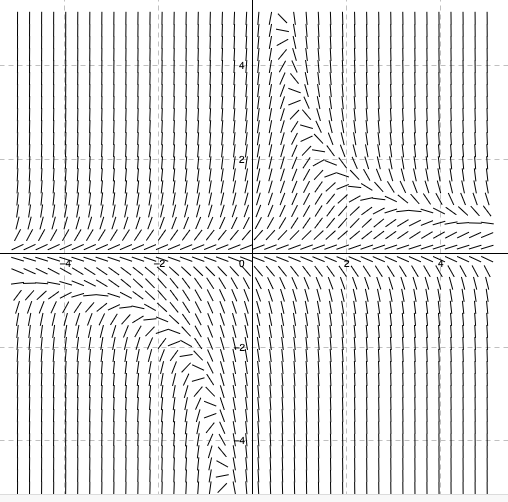
\includegraphics[width=.9\linewidth]{./14.png}
\end{center}

Based on the direction field and on the differential equation, for \(y_0 < 0\),
the slopes eventually become negative, therefore tend to \(-\infty\). If
\(y_0=0\), then we get an equilibrium solution. Note that slopes are zero along
the curves \(y=0\) and \(ty = 3\).

\subsection*{Problem 16}
\label{sec:org84aea3a}
\begin{center}
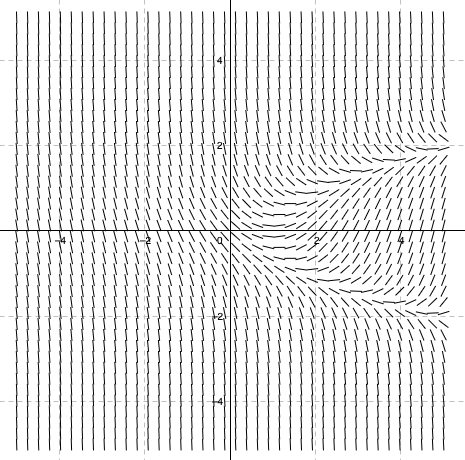
\includegraphics[width=.9\linewidth]{./16.png}
\end{center}

Solutions with \(t_{0}<0\) all tend to \(-\infty\). Solutions with initial
conditions \(\left(t_{0}, y_{0}\right)\) to the right of the parabola
\(t=1+y^{2}\) asymptotically approach the parabola as
\(t \rightarrow \infty\).
Integral curves with initial conditions above the parabola (and
\(\left.y_{0}>0\right)\) also approach the curve. The slopes for solutions with
initial conditions below the parabola (and \(\left.y_{0}<0\right)\) are all
negative. These solutions tend to \(-\infty\).

\subsection*{Problem 27 [FOR GRADE]}
\label{sec:org4242b51}
The solution of the initial value problem
\begin{equation*}
  y_1'+2y_1=0, \quad y_1(0) = 1
\end{equation*}
is \(y_1(t) = e^{-2t}\). Therefore by approaching to \(1\) from the left side
(\(1^-\) notation), we get \(y(1^-) = y_1(1) = e^{-2}\). On the interval \((1,
   \infty)\), the differential equation is \(y_2'+y_2=0\) with
\(y_2(t)=ce^{-t}\). Therefore by approaching \(1\) from the right side
(notationally \(1^+\)), we see \(y(1^+)=y_2(1)=ce^{-1}\). Equating both the
limits of the function
\begin{align*}
  y(1^-) = y(1^+) \iff c = e^{-1}
\end{align*}
Therefore the global solution is
\begin{equation*}
  y(t) = 
  \begin{cases}
    e^{-2t}, \quad 0 \leq t \leq 1\\
    e^{-1-t}, \quad t > 1
  \end{cases}
\end{equation*}

\subsection*{Problem 28}
\label{sec:org714f839}
The Eleventh Edition (latest) of the book doesn't have this problem.

\section*{Section 2.6}
\label{sec:orge2a6e6a}

\subsection*{Problem 3 [FOR GRADE]}
\label{sec:orgaac2640}
They have the form \(M(x,y) + N(x,y) \frac{dy}{dx} = 0\). So
\begin{align*}
  M(x,y) = 3x^2-2xy+2 \quad \text{and} \quad N(x,y) = 6y^2-x^2+3
\end{align*}
Then we see \(\frac{\partial M}{\partial y} = -2x\) and \(\frac{\partial
   N}{\partial x} = -2x\). Therefore, our equation is of exact form. So our
solution \(F_x = M \implies F = \int M dx = x^3 - x^2y + 2x + g(y)\).
Then
\begin{equation*}
F_y = -x^2+g'(y) = N \implies g'(y) = 6y^2+3 \implies g(y)=2y^3 + 3y
\end{equation*}
Finally,
\begin{equation*}
  F = x^3 - x^2y + 2x +2y^3 + 3y = C
\end{equation*}

\subsection*{Problem 5}
\label{sec:org0fe7a9e}
\begin{align*}
  \frac{dy}{dx} = - \frac{ax-by}{bx-cy} \\
  \iff (ax-by)dx + (bx-cy)dy = 0
\end{align*}
Now, \(M = ax-by\) and \(N = bx -cy\). See that
\begin{align*}
  M_y = -b \neq N_x = b
\end{align*}
The differential equation is not exact.

\subsection*{Problem 13}
\label{sec:orgddc8a73}
Integrating \(\psi_{y}=N\), while holding \(x\) constant, yields \(\psi(x, y)=\int
N(x, y) d y+h(x)\) 
Taking the partial derivative with respect to
\(x, \psi_{x}=\int \frac{\partial}{\partial x} N(x, y) d y+h^{\prime}(x)\) .
Now set \(\psi_{x}=M(x,
y)\) and therefore
\(h^{\prime}(x)=M(x, y)-\int \frac{\partial}{\partial x} N(x,y) dy\).
Based on the fact that \(M_{y}=N_{x}\), it follows that
\(\frac{\partial}{\partial y}\left[h^{\prime}(x)\right]=0\). Hence the expression
for \(h^{\prime}(x)\) can be integrated to obtain 
\begin{align*}
h(x)=\int M(x, y) d x-\int\left[\int \frac{\partial}{\partial x} N(x, y) d y\right] d x
\end{align*}

\subsection*{Problem 15 [FOR GRADE]}
\label{sec:orgdcc6856}
\begin{align*}
  M = x^2y^3,\quad \quad N = x(1+y^2)\\
  \implies M_y = 3x^2y^2, \quad \quad N_x = 1+y^2
\end{align*} 
Trivially, not exact. Let \(\mu(x,y) = \frac{1}{xy^3}\),
then
\begin{align*}
  M\times\mu = x, \quad \quad N\times\mu = \frac{1+y^2}{y^3}
  \implies (M\times\mu)_y = 0, \quad \quad (N\times\mu)_x = 0
\end{align*}
Now they're exact! 

So then just find that \(F = \frac{x^2}{2} - \frac{1}{2y^2}+\ln(y)\)

\subsection*{Problem 18}
\label{sec:org2102992}
\begin{align*}
  M = 3x^2y+2xy+y^3,\quad \quad N = x^2+y^2\\
  \implies M_y = 3x^2+2x+3y^2, \quad \quad N_x = 2x
\end{align*} 
Let us find the integrating factor
\begin{align*}
  \mu(y) &= \exp\left(\int \frac{M_y-N_x}{N} dx\right)\\
         &= \exp\left(\int \frac{3x^2+2x+3y^2-2x}{x^2+y^2} dx\right)\\
         &= \exp\left(\int 3 dx\right)\\
         &= e^{3x}
\end{align*}
Simply confirm that \(M\mu\) and \(N\mu\) are now exact.
Find \(F(x,y) = e^{3x}y(3x^2+y^2) = C\)
\end{document}